\documentclass{beamer}
%
% Choose how your presentation looks.
%
% For more themes, color themes and font themes, see:
% http://deic.uab.es/~iblanes/beamer_gallery/index_by_theme.html
%
\mode<presentation>
{
  \usetheme{Warsaw}      % or try Darmstadt, Madrid, Warsaw, ...
  \usecolortheme{default} % or try albatross, beaver, crane, ...
  \usefonttheme{default}  % or try serif, structurebold, ...
  \setbeamertemplate{navigation symbols}{}
  \setbeamertemplate{caption}[numbered]
} 

\usepackage{lmodern}
\usepackage[T1]{fontenc} 
\usepackage{microtype}
\usepackage{inconsolata}
\usepackage[icelandic,english]{babel}
\selectlanguage{english}
\usepackage[utf8x]{inputenc}
\usepackage{amsmath}
\usepackage{amsfonts}
\usepackage{mathtools}
\usepackage{amssymb}
\usepackage{amsthm}
\usepackage{xcolor,colortbl}
\usepackage{caption}
\usepackage{subcaption}
\usepackage{etoolbox}
\usepackage{graphicx}
\usepackage{tikz}
\usepackage{verbatim}
\usepackage{listings}
\lstdefinestyle{java-dark}
{	
    backgroundcolor=\color{black},
    commentstyle=\color{gray},
    keywordstyle=\color{red},
    numberstyle=\tiny\color{black},
    stringstyle=\color{green},
    identifierstyle=\color{orange},
	basicstyle=\scriptsize\ttfamily\color{white},
    breakatwhitespace=false,
    breaklines=true,
    captionpos=b,
    keepspaces=true,
    numbers=left,
    numbersep=5pt,
    showspaces=false,
    showstringspaces=false,
    showtabs=false,
    tabsize=2,
}

\newcommand{\B}{\mathbb{B}} % binary set
\newcommand{\N}{\mathbb{N}} % set of natural numbers
\newcommand{\Z}{\mathbb{Z}} % set of integers 
\newcommand{\Q}{\mathbb{Q}} % set of rationals
\newcommand{\R}{\mathbb{R}} % set of reals
\newcommand{\C}{\mathbb{C}} % set of complex
\newcommand{\map}[3]{#1: #2 \to #3} % 1 : 2 -> 3
\newcommand{\der}[1]{\frac{d}{d#1}} % derivative
\newcommand{\set}[1]{\left\{#1\right\}} % set, general
\newcommand{\nset}[1]{\set{1,2,\ldots,#1}} % {1,2,...,n}
\newcommand{\cata}[1]{\frac{1}{#1+1}\binom{2#1}{#1}} % catalan numbers
\renewcommand{\vector}[1]{(x_1,x_2,\ldots,x_{#1})} % x-vector, len n
\newcommand{\avector}[2]{(#1_1,#1_2,\ldots,#1_{#2})} % ?-vector, len n
\newcommand{\vvec}[1]{\begin{pmatrix}#1\end{pmatrix}}
\newcommand{\mc}[1]{\mathcal{#1}}
\newcommand{\ttt}[1]{\texttt{#1}}
\newcommand{\ilim}[1]{\lim_{#1\to\infty}}
\newcommand{\bpar}[1]{\left(#1\right)}
\newcommand{\floor}[1]{\left\lfloor #1 \right\rfloor}

\title[Game Engine Architecture]{Mesh Generator}
\author{Jón Steinn Elíasson}
\institute{Reykjavík University}
\date{\today}

\begin{document}

\begin{frame}
  \titlepage
\end{frame}

\section{Introduction}
\begin{frame}{Introduction}
\begin{itemize}
\item Mesh generated with mathematical functions
\item Generate fixed noise surfaces
\item UI to preview and download as \texttt{.obj}
\end{itemize}
\begin{figure}
\includegraphics[scale=0.5]{terrain.png}
\end{figure}
\end{frame}

\section{Motivation and purpose}
\begin{frame}{Motivation/Purpose}
\begin{itemize}
\item The idea is from prior year's particle exporters
\begin{itemize}
\item I still wanted to do something different
\end{itemize}
\item Can create more complicated 'primitive' objects
\item Good for math function visualization
\item Can create fixed terrain
\end{itemize}
\end{frame}

\section{Existing work}
\begin{frame}{Existing work}
\begin{itemize}
\item Many mathematical software provide 3D rendering of functions
\begin{itemize}
\item SageMath
\item Mathematica
\item Matlab
\end{itemize}
\item Most do not allow free travel when exploring
\item Have not found one with \texttt{.obj} exporter.
\end{itemize}
\end{frame}
\begin{frame}
\begin{itemize}
\item Compared to SageMath
\end{itemize}
\begin{figure}
\includegraphics[scale=0.45]{existing.png}
\end{figure}
\end{frame}

\section{My Contribution}
\begin{frame}{What I used}
\begin{figure}
\begin{tikzpicture}
\draw (0,0) node {\includegraphics[scale=0.1]{flask-logo.png}};
\draw (3,1) node {\includegraphics[scale=0.5]{noise-logo.png}};
\draw (3,-1) node {\includegraphics[scale=0.2]{py-logo.png}};
\draw (-3,-1) node {\includegraphics[scale=0.1]{threejs-logo.png}};
\draw (-3,1) node {\includegraphics[scale=0.1]{webgl-logo.png}};
\end{tikzpicture}
\end{figure}
\end{frame}

\begin{frame}{What I did}
\begin{itemize}
\item Web GUI 
\item Example rendering and exploring in WebGL
\item Three different type of generation
\begin{itemize}
	\item Map the $xz$-plane to a height point
    \item Map a $uv$-plane to 3D space
    \item Map the $xz$-plane to height point with noise
\end{itemize}
\item Objects include
\begin{itemize}
	\item Vertices
    \item Normals
    \item Texture coordinates
    \item Faces
\end{itemize}
\end{itemize}
\end{frame}
\begin{frame}{A mapping example}
\begin{figure}
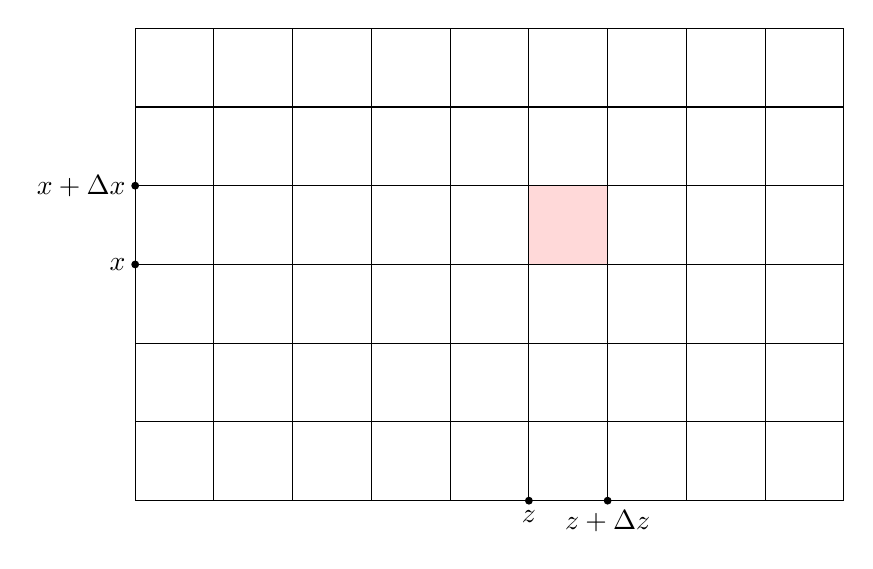
\begin{tikzpicture}
\fill[red!15] (5,3) rectangle (6,4);
\draw (0,0) grid (9,6);
\fill (5,0) circle (0.05);
\fill (6,0) circle (0.05);
\fill (0,3) circle (0.05);
\fill (0,4) circle (0.05);
\draw (5,0) node[below] {$z$};
\draw (6,0) node[below] {$z+\Delta z$};
\draw (0,3) node[left] {$x$};
\draw (0,4) node[left] {$x + \Delta x$};
\end{tikzpicture}
\end{figure}
\end{frame}
\begin{frame}{A mapping example}
\begin{figure}
\begin{tikzpicture}
\draw (0,0) rectangle (4,4);
\fill (0,0) circle (0.05) node[below left] {\tiny $\left(x,f(x,z),z\right)$};
\fill (0,4) circle (0.05) node[above left] {\tiny $\left(x+\Delta x,f(x+\Delta x,z),z\right)$};
\fill (4,0) circle (0.05) node[below right] {\tiny $\left(x,f(x,z+\Delta z),z + \Delta z\right)$};
\fill (4,4) circle (0.05) node[above right] {\tiny $\left(x+\Delta x,f(x+\Delta x,z+\Delta z),z+\Delta z\right)$};
\draw[dotted] (0,0) -- (4,4);
\end{tikzpicture}
\end{figure}
\end{frame}

\end{document}
